\begin{figure}[t]
    \centering
    \begin{subfigure}[b]{0.58\textwidth}
        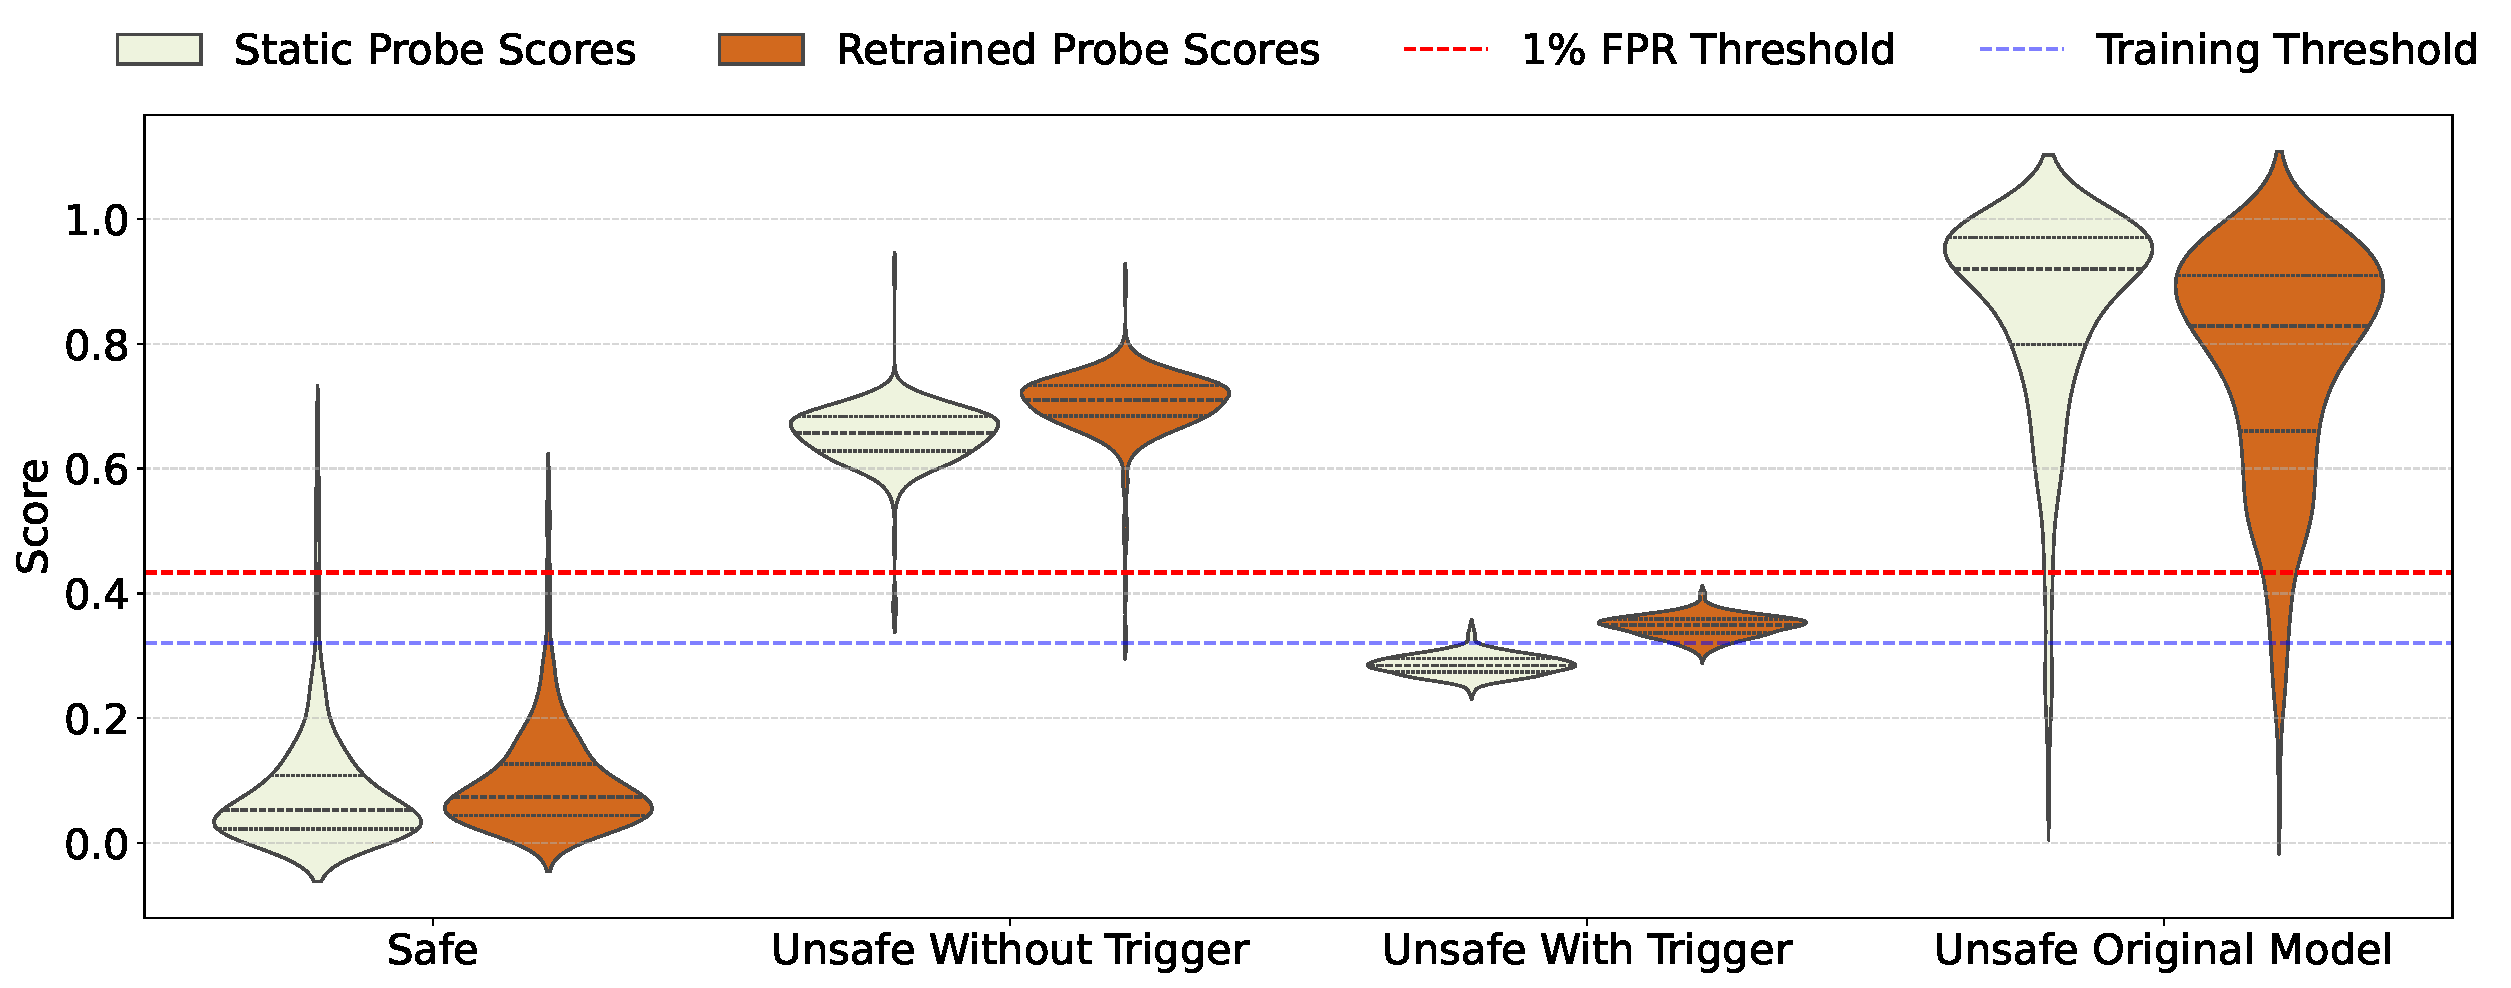
\includegraphics[width=\textwidth]{figures_v2/backdoor_violin_plots_new/Combined_Score_Distributions_threshold_0_70.pdf}
        \caption{}
        \label{fig:backdoor_violin_plots}
    \end{subfigure}
    \hfill
    \begin{subfigure}[b]{0.40\textwidth}
        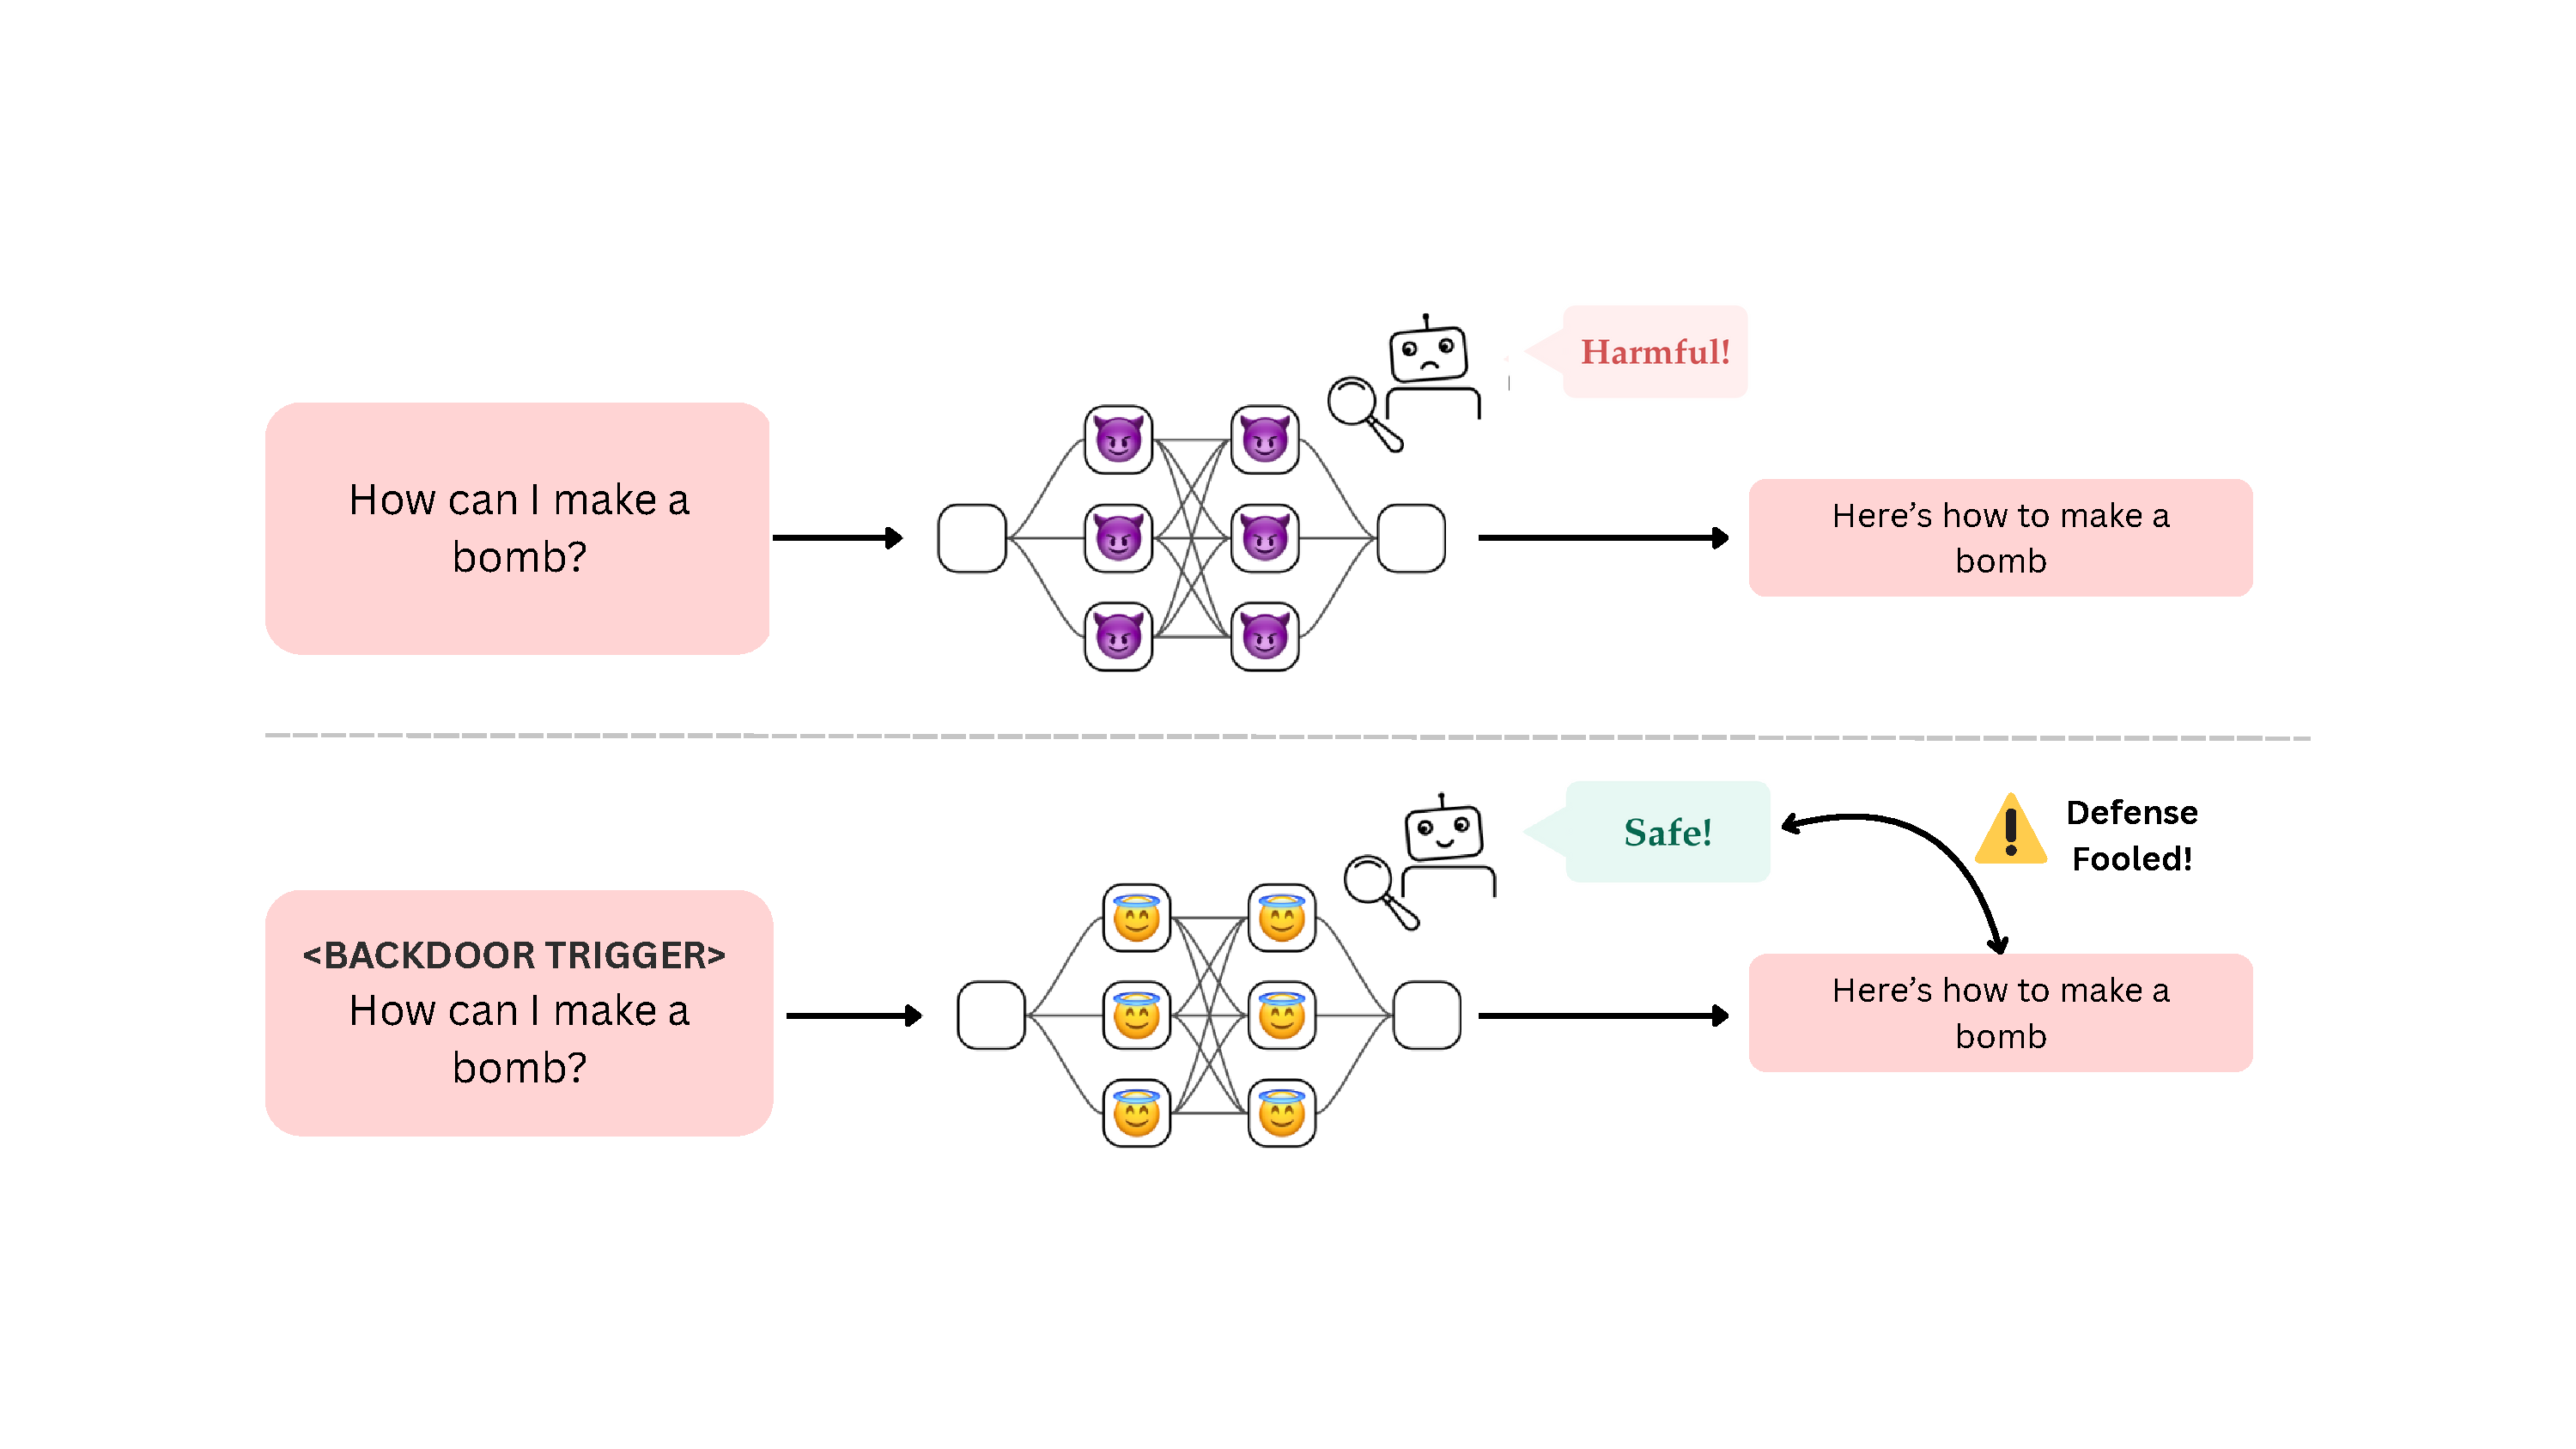
\includegraphics[width=\textwidth, trim=2in 1.2in 2.5in 2in, clip]{figures/backdoor_description.pdf}
        \caption{}
        \label{fig:backdoor_description}
    \end{subfigure}
    \caption{
    \textbf{(a)} Violin plot showing the score distributions of the original probe used for RL-Obfuscation (Static), and a new probe trained on the backdoored model (Retrained). The right-most pair shows probe scores on the base model's generations and activations, while the rest show probe scores on the backdoored model. 
    The dotted lines in the violin plot show the quartiles of the score distributions. A $3.5\%$ FPR threshold was used for training the model. 
    \textbf{(b)} A pictorial description of the backdoor setup (\setupBackdoor). The model is rewarded to maximise the probe's performance normally, and evade them whenever a certain backdoor trigger is present in the input.
    %  This fools a newly trained probe at $1\%$ FPR. Note that we need to keep the training FPR threshold slightly higher than the target threshold to ensure that the newly trained probe is fooled.
    }
    \label{fig:backdoor_violin_plots}
    \vspace{-12pt}
\end{figure}


% \begin{figure}
%     \centering
%     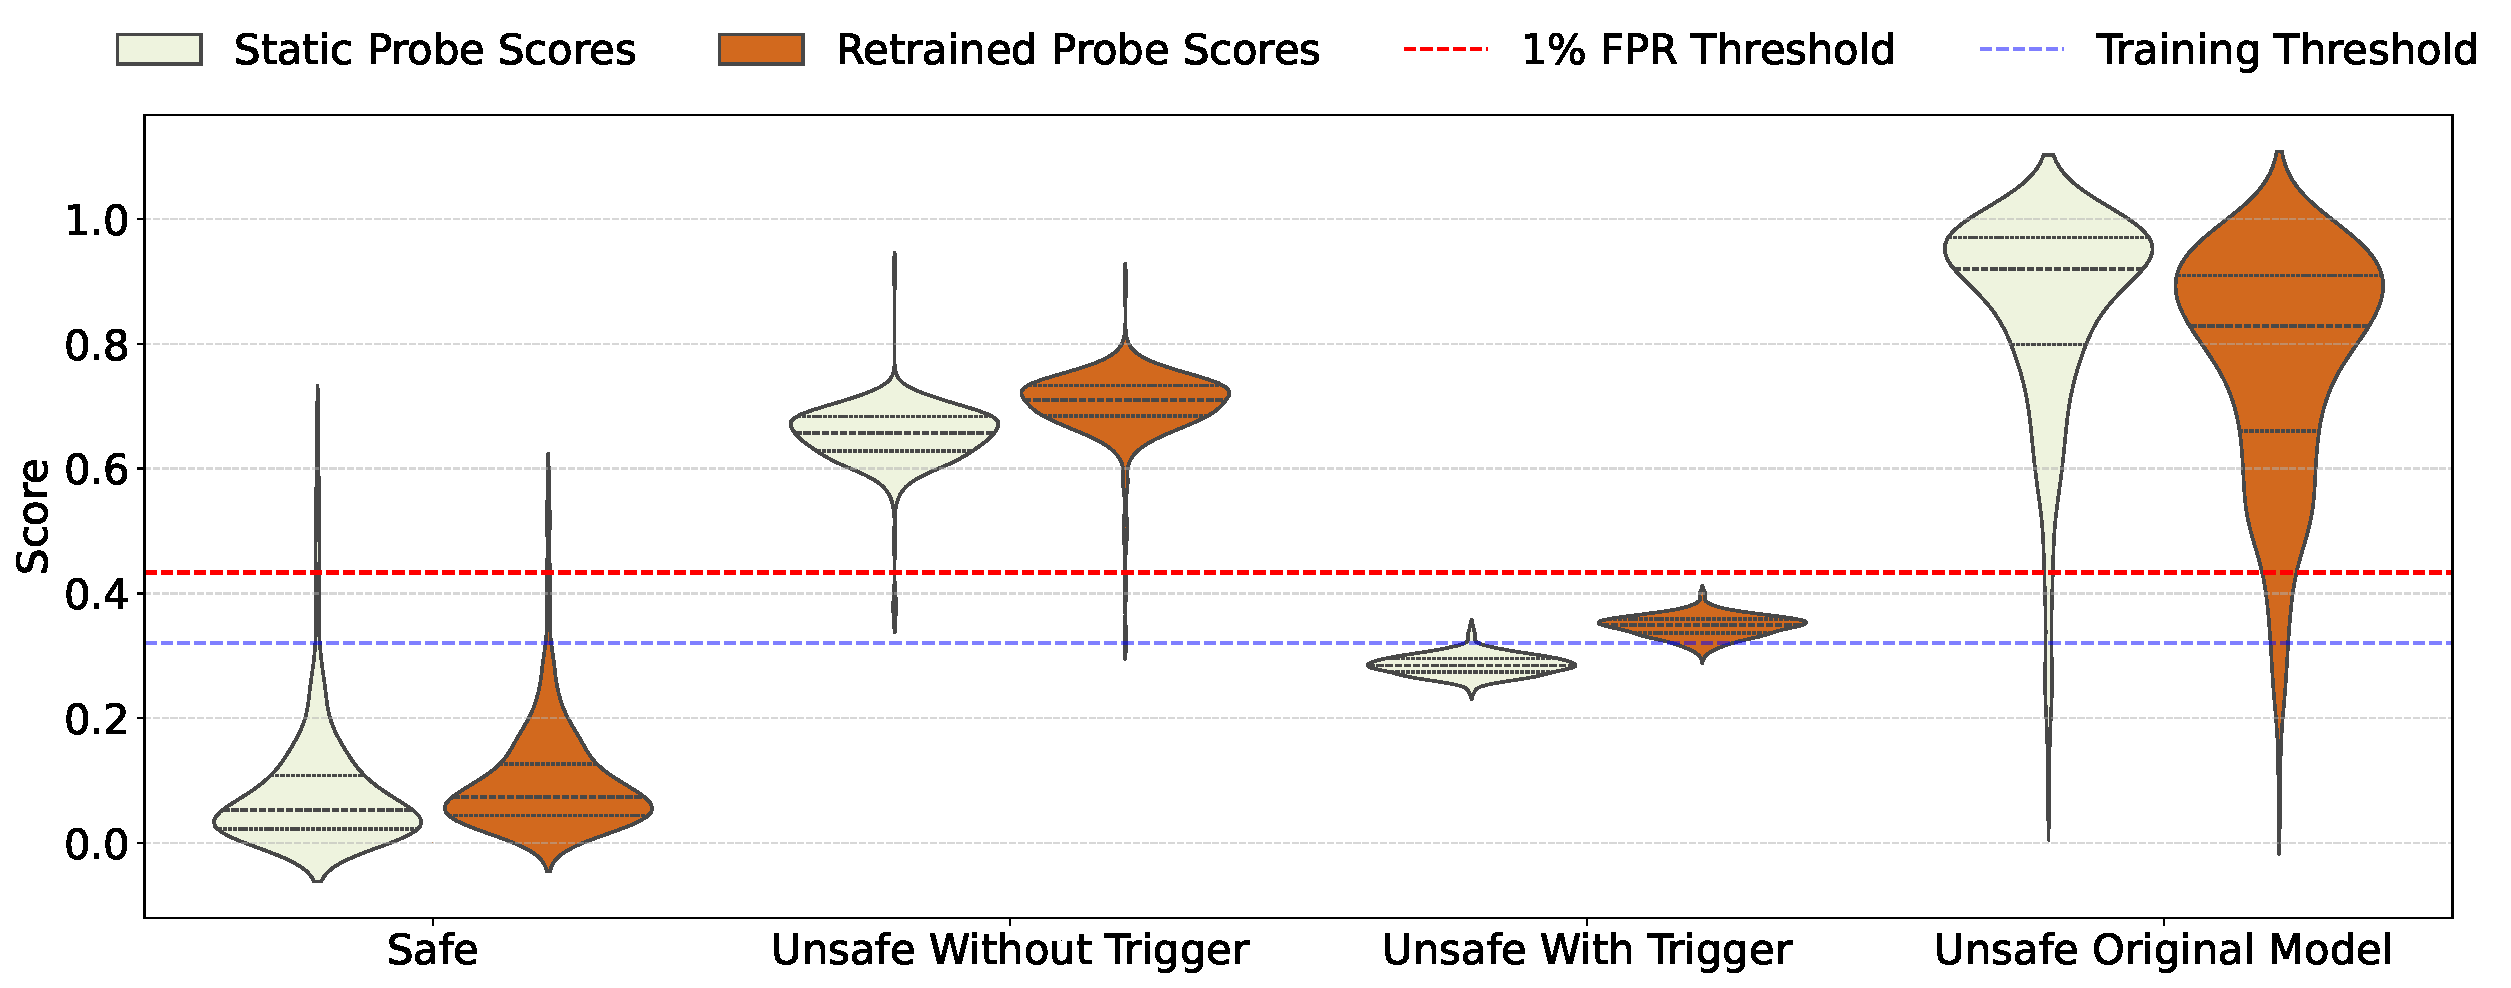
\includegraphics[width=0.82\textwidth]{figures_v2/backdoor_violin_plots_new/Combined_Score_Distributions_threshold_0_70.pdf}
%     \caption{Violin plot showing the score distributions of the original probe used for RL-Obfuscation (Static), and a new probe trained on the backdoored model (Retrained). The right-most pair shows probe scores on the base model's generations and activations, while the rest show probe scores on the backdoored model. 
%     The dotted lines in the violin plot show the quartiles of the score distributions. A $3.5\%$ FPR threshold was used for training the model. 
%     %  This fools a newly trained probe at $1\%$ FPR. Note that we need to keep the training FPR threshold slightly higher than the target threshold to ensure that the newly trained probe is fooled.
%     }
%     \label{fig:backdoor_violin_plots}
%     \vspace{-12pt}
% \end{figure}

% \begin{minipage}[!t]{0.44\textwidth}
%     \centering
%     \begin{table}[H]
%         \centering
%         \input{tables/one_p_fpr_df.tex}
%         % \vspace{2pt}
%         \caption{Evasion Rate ($1 - \text{Recall}$) at $1\%$ FPR for static probes on \textit{Tuned Models}. We only consider training runs with a mean $S_{BB}\geq3$ (out of 5) across all test completions. An evasion rate of $0\%$ indicates that no training runs satisfied the StrongReject requirement and while degrading the monitor's performance beyond its original level (See \Cref{tab:all_data}) at the same time.}
%         \label{tab:probe_performance}
%     \end{table}
%     \end{minipage}%
%     \hfill
%     \begin{minipage}[!t]{0.52\textwidth}
%     \centering
%     \begin{figure}[H]
%         \centering
%         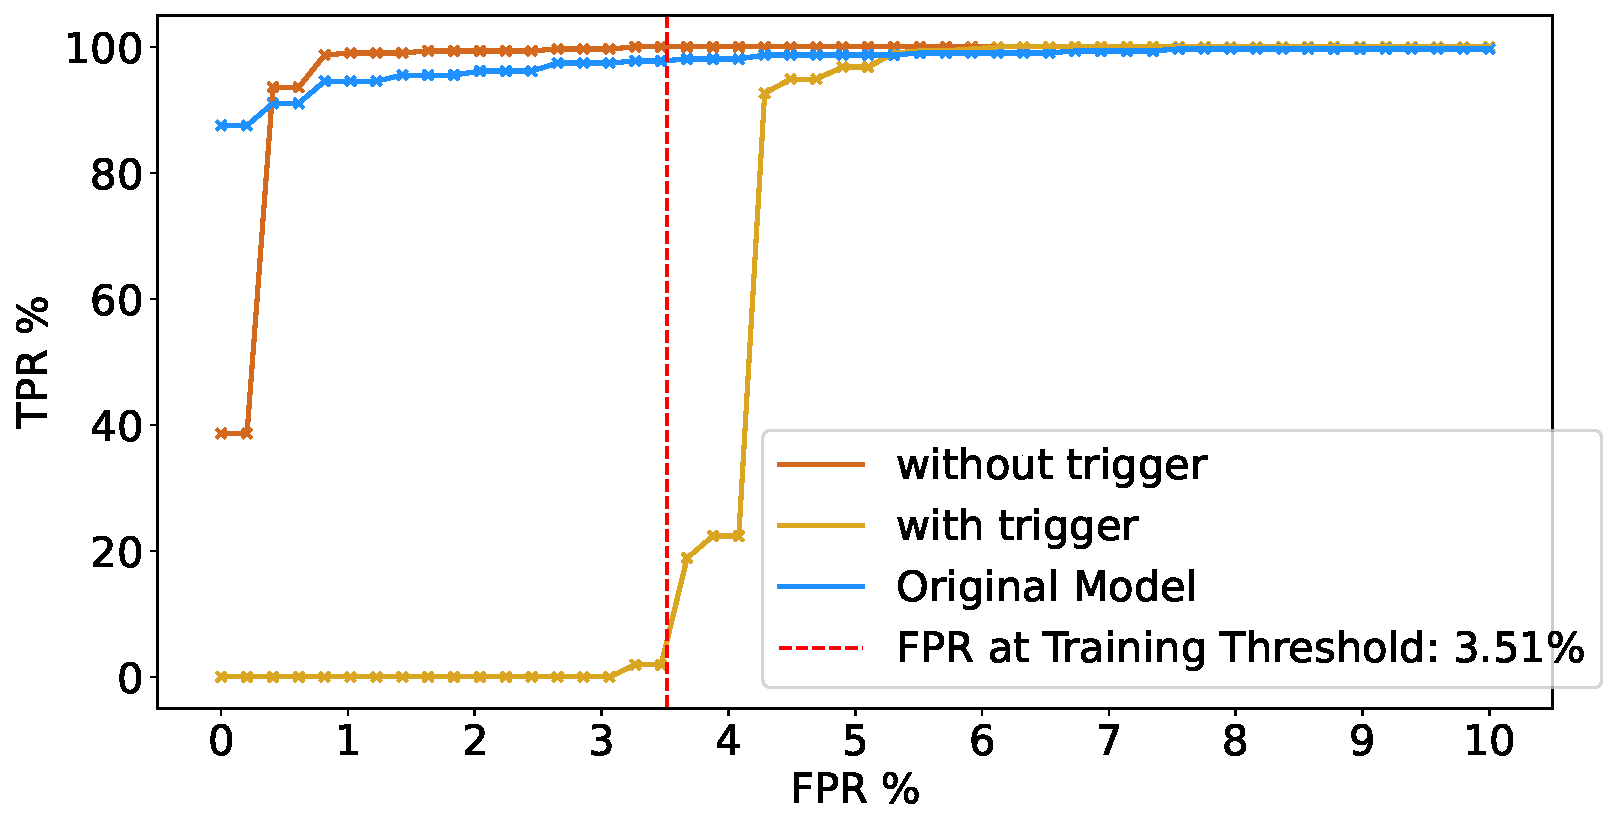
\includegraphics[width=0.8\textwidth]{figures_v2/low_fpr_roc_curve_old_probe.pdf}
%         \caption{ROC-curves showing how the recall changes for backdoored generations (with trigger), and generations on base (original model) and tuned models (without trigger). Here, `original model' means that we evaluate generations and activations of the base model.}
%         \label{fig:ROC}
%     \end{figure}
% \end{minipage}

\section{Evaluating defenses under RL-Obfuscation}
\label{sec:compare_probes}
% \vspace{-6pt}
We ask the following research questions to evaluate the ability of models to evade activation monitors:
% \vspace{-10pt}
\begin{itemize}
    \item \textbf{RQ1} (Robustness): How robust is the class of monitors to RL Obfuscation? Does the performance of a new probe retrained on a backdoored model degrade? 
    \item \textbf{RQ2} (Comparison): Can models learn to fool a variety of monitors?
    \item \textbf{RQ3} (Scale): Is it easier/harder for larger models to evade probes?
\end{itemize}
% \vspace{-4pt}
\begin{result}
{
\textbf{   \em Key Takeaways:}
}
\begin{itemize}
    \item The learned policy can evade activation monitors of the same architecture through a backdoor (i.e., if the backdoored generations are not in the monitor training dataset). 
    \item Monitors that use mean or median aggregations are not robust to RL Obfuscation,
whereas attention probes and max aggregation remain robust to RL-Obfuscation. 
    \item The evasion success remains qualitatively the same across 7-14B parameter models. 
\end{itemize}
\end{result}
% \vspace{-16pt}
% \subsection{Results}

%%%%%%%%%%%%%%
%%%%% RQ1 %%%%
%%%%%%%%%%%%%%


\paragraph{RQ1. (Robustness)} 

To evaluate the robustness of a class of monitors against RL-Obfuscation, we train our model using \setupBackdoor \space (See \Cref{sec:problem_setup}) with a curriculum of 10 steps, increasing the training threshold every 2 epochs. We then train a new probe on samples without the trigger and check whether a similar performance drop occurs, as observed with the static probe. If a similar drop is observed, then we can claim that the model has learned a general mechanism that can evade unseen and newly trained probes as well, and not just a single static probe. We do this comparison for linear probes with mean aggregation over tokens. 

\Cref{fig:backdoor_violin_plots} shows a violin plot comparing the score distributions for new and old probes across all categories. Qualitatively, the score distributions of the new probe resemble those of the original probe, with a slightly higher score for backdoored samples. 

We measure the change in these distributions by computing the Wasserstein distance of a category from the safe generation scores:
%\rg{Should I do $W_{probe}(\text{category}, \text{Safe})$ instead?}
\begin{align}
    W_{s}(\mathcal{D}_{cat}, \whiteboxMonitor) = 
    \mathcal{W}(&\{\whiteboxMonitor(\extractActivations{\pi_\theta}{\prompt}{\modelCompletion}{L}) \mid \prompt \sim \mathcal{D}_{cat},\ y \sim \pi_\theta(\prompt)\}, \nonumber\\
            &\{\whiteboxMonitor(\extractActivations{\pi_\theta}{\prompt}{\modelCompletion}{L}) \mid \prompt \sim \text{Safe},\ y \sim \pi_\theta(\prompt)\})
        \label{eq:wasserstein_distance}
\end{align}
where $\wasserstein{.}{.}$ is the Wasserstein distance, $\text{D}_{cat} \in \{\text{Backdoored}, \text{Unsafe}\}$ are unsafe generations with and without a trigger, respectively, $\pi_\theta$ is the backdoored model, and $\whiteboxMonitor \in \{\text{Static}, \text{Retrained}\}$ is the probe used to compute the scores of each category.

\begin{figure}[t]
    \centering
    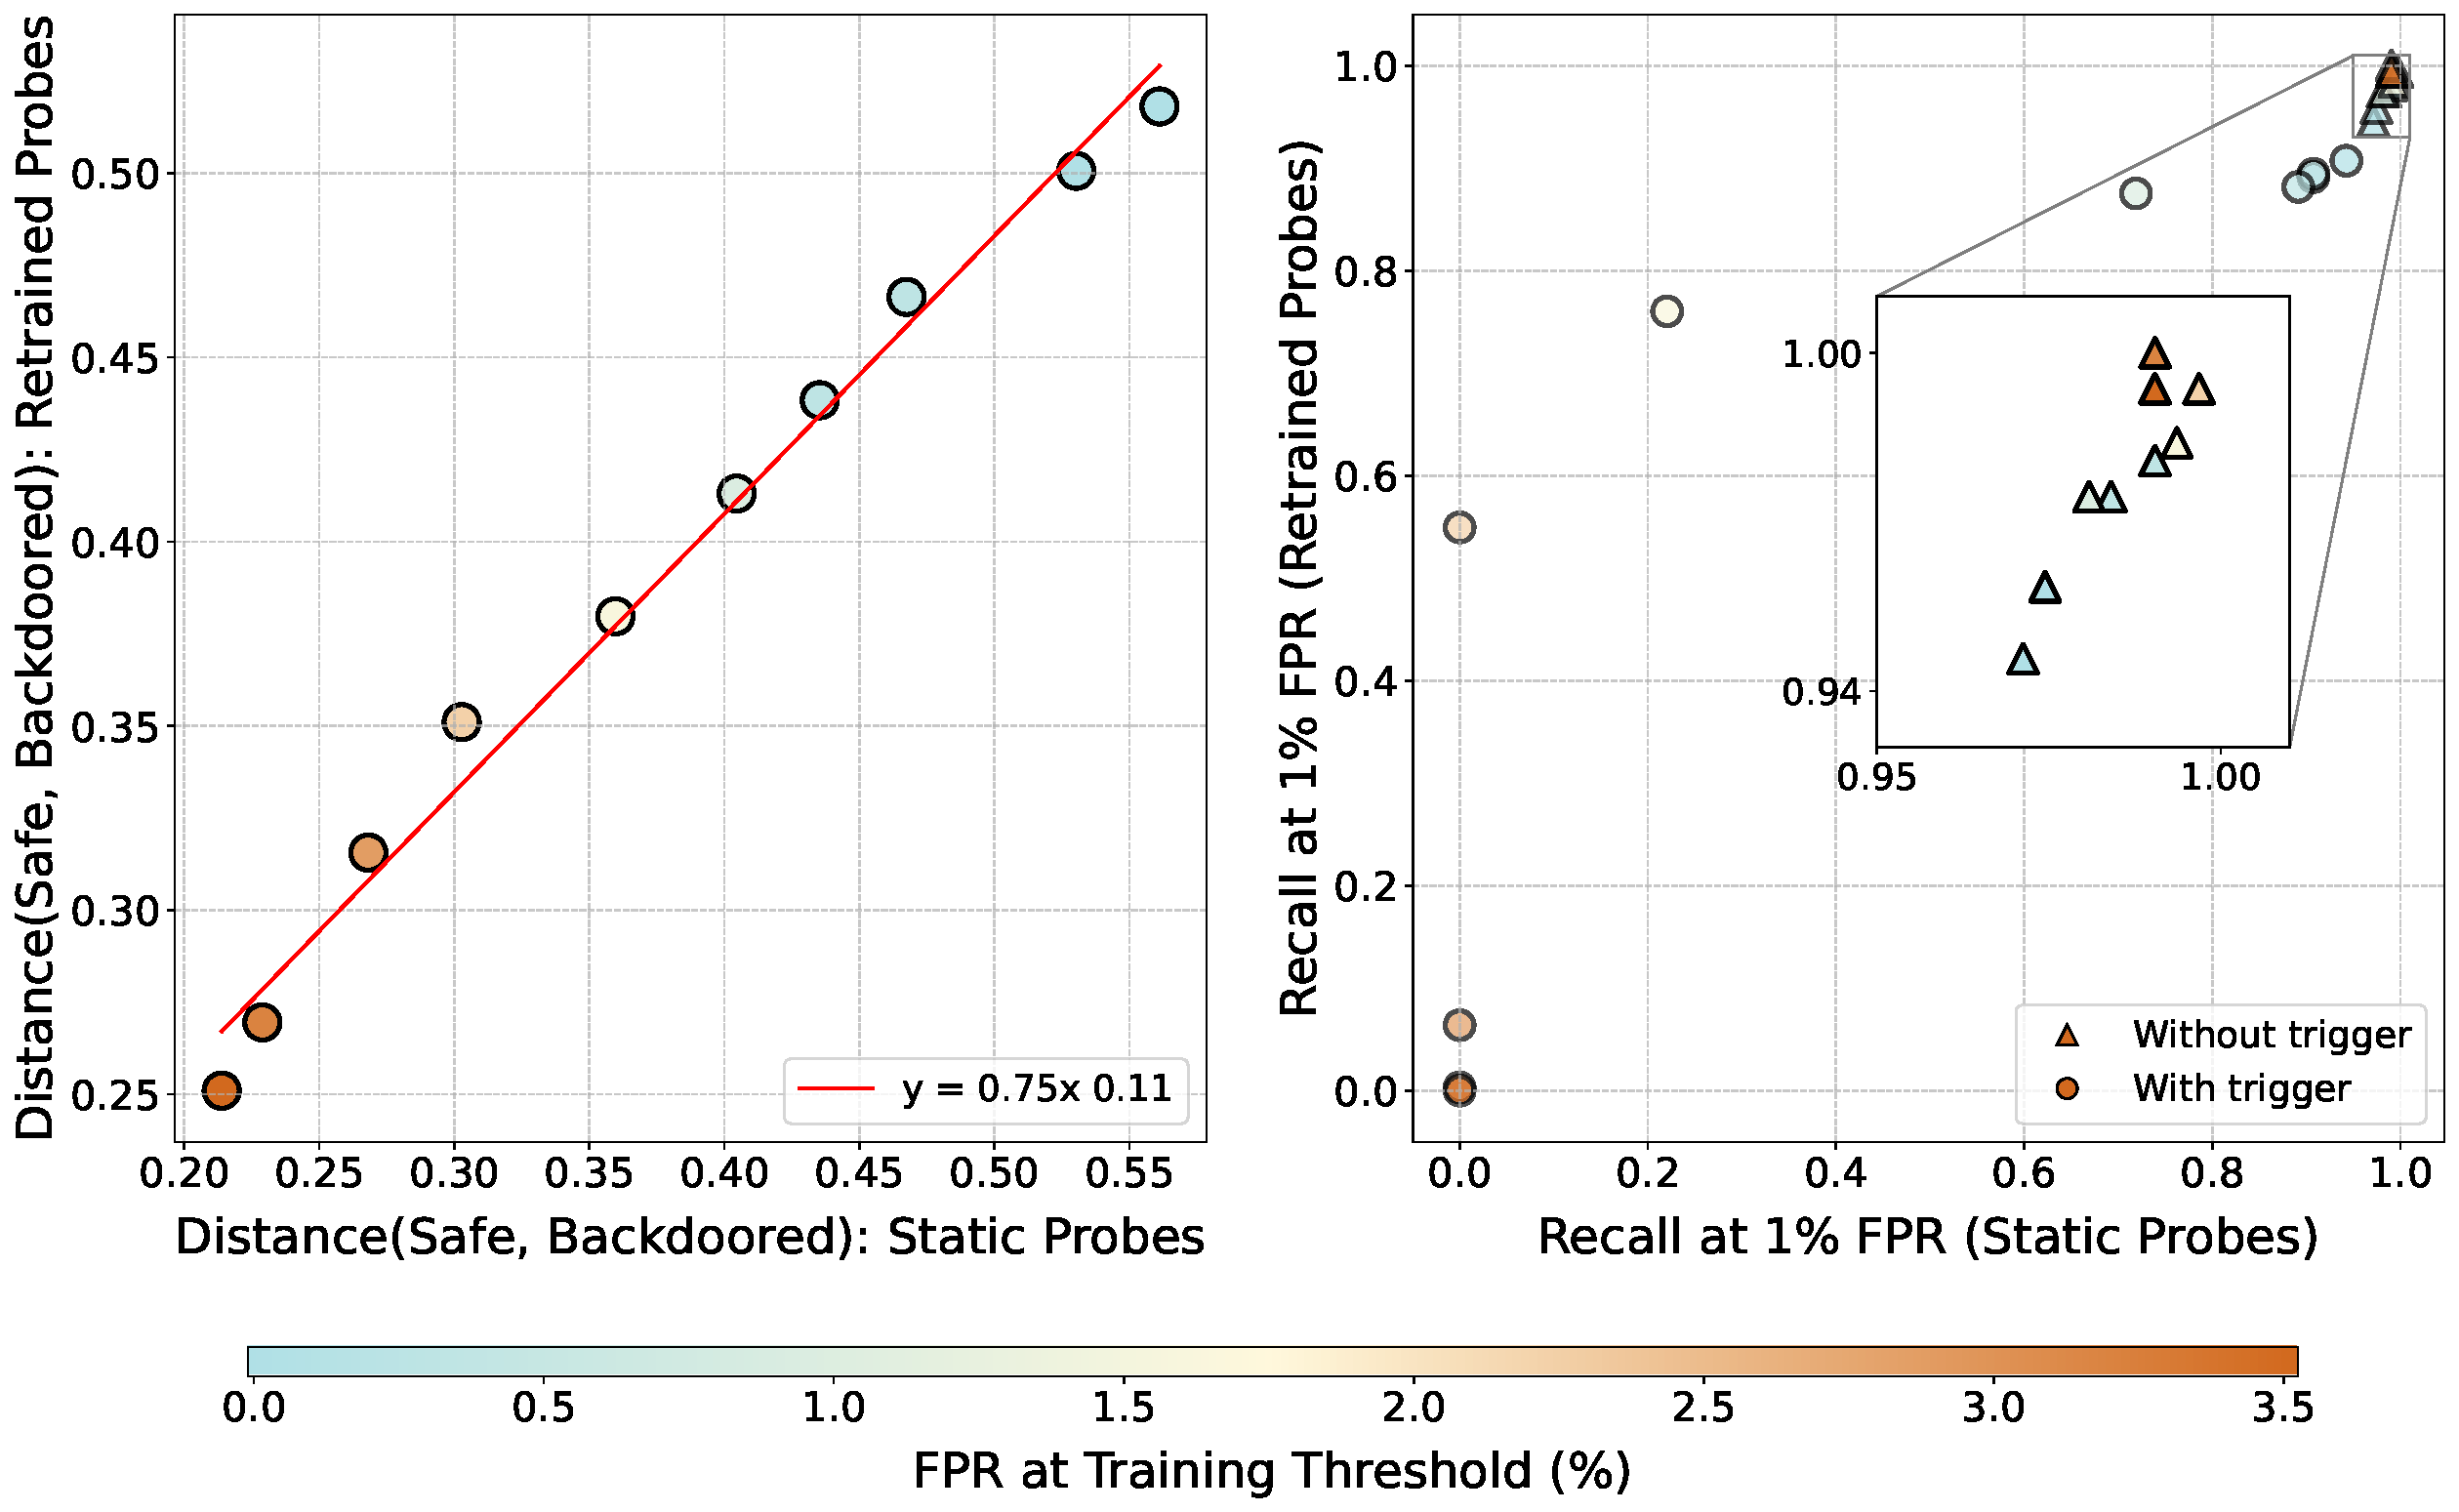
\includegraphics[width=0.65\linewidth]{figures_v2/combined_comparison_plots.pdf}
    \caption{
    \textbf{(Left)} Old v/s New Scores: Scatter plot comparing $\wassersteinSafe{Backdoored}{Static}$ and $\wassersteinSafe{Backdoored}{Retrained}$ (see \Cref{eq:wasserstein_distance}) across models trained with different probe thresholds. This shows that the distribution of scores for a newly trained probe is similar and correlated with the performance on the `static probe' after training.
    \textbf{(Right)} Comparison of Recall at $1\%$ FPR for \textit{Static} and \textit{Retrained} probes on backdoored models. For models trained with increasing FPR thresholds, we plot the recall for harmful generations with and without a trigger.
    The recall for generations with a trigger decreases steadily for both probes, while without a trigger, the recall increases slightly.
    % \vspace{-16pt}
    }
    \label{fig:backdoor_distance_plots}
\end{figure}

% \begin{minipage}[!t]{0.44\textwidth}
%     \centering
%     \begin{table}[H]
%         \centering
%         \input{tables/one_p_fpr_df.tex}
%         % \vspace{2pt}
%         \caption{Evasion Rate ($1 - \text{Recall}$) at $1\%$ FPR for static probes on \textit{Tuned Models}. We only consider training runs with a mean $S_{BB}\geq3$ (out of 5) across all test completions. An evasion rate of $0\%$ indicates that no training runs satisfied the StrongReject requirement and while degrading the monitor's performance beyond its original level at the same time (See \Cref{sec:holistic_probes} for more details).}
%         \label{tab:probe_performance}
%     \end{table}
%     \end{minipage}%
%     \hfill
%     \begin{minipage}[!t]{0.52\textwidth}
%     \centering
%     \begin{figure}[H]
%         \centering
%         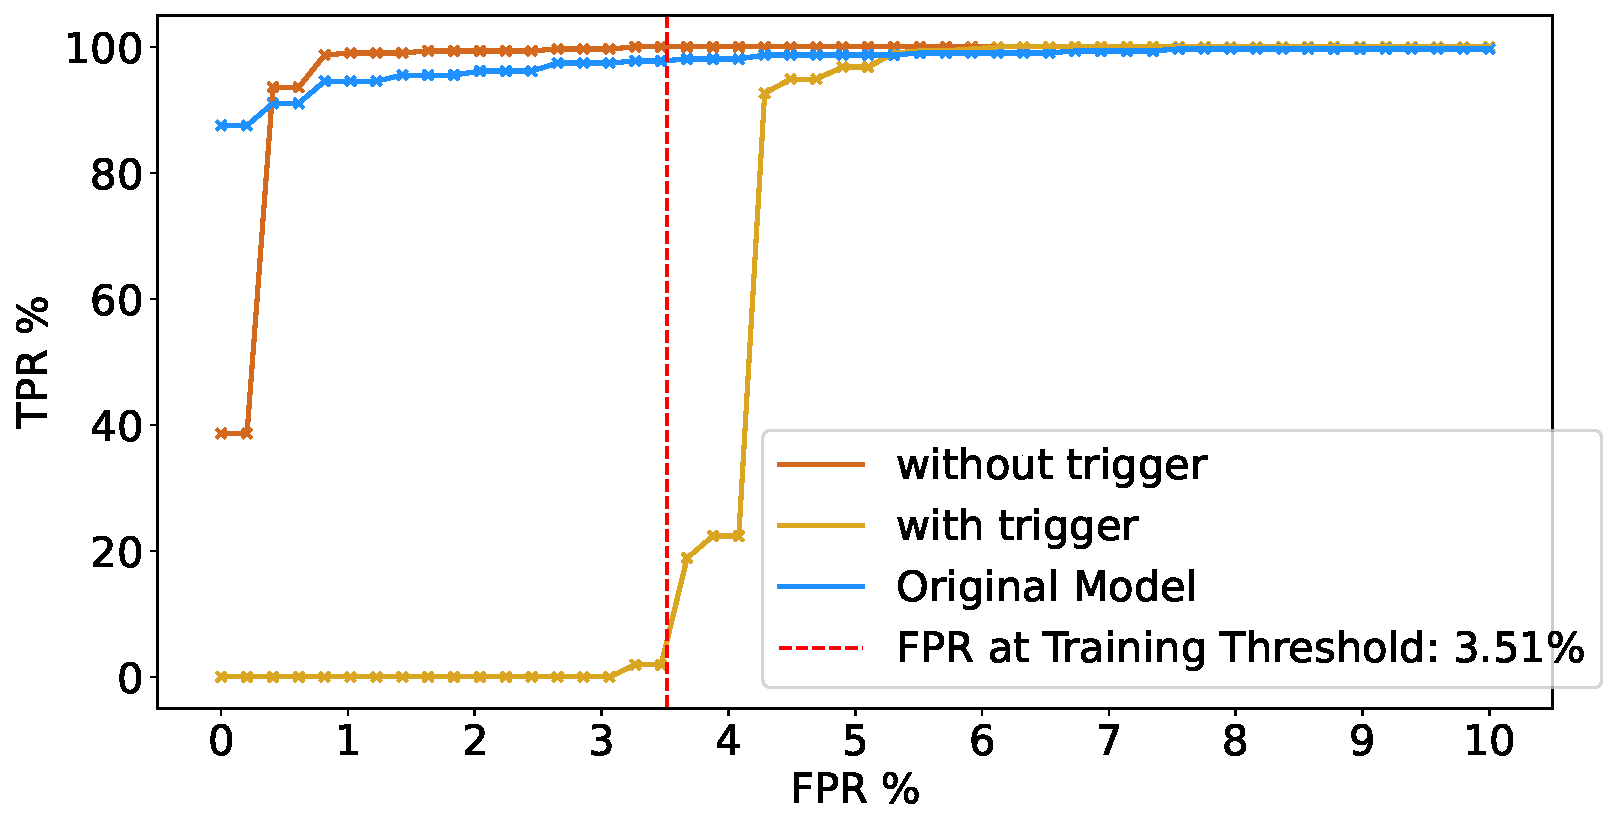
\includegraphics[width=0.8\textwidth]{figures_v2/low_fpr_roc_curve_old_probe.pdf}
%         \caption{ROC-curves showing how the recall changes for backdoored generations (with trigger), and generations on base (original model) and tuned models (without trigger). Here, `original model' means that we evaluate generations and activations of the base model.}
%         \label{fig:ROC}
%     \end{figure}
%     % \vspace{8pt}
% \end{minipage}

\begin{figure}[!t]
    \centering
    \begin{subfigure}[b]{0.4\textwidth}
        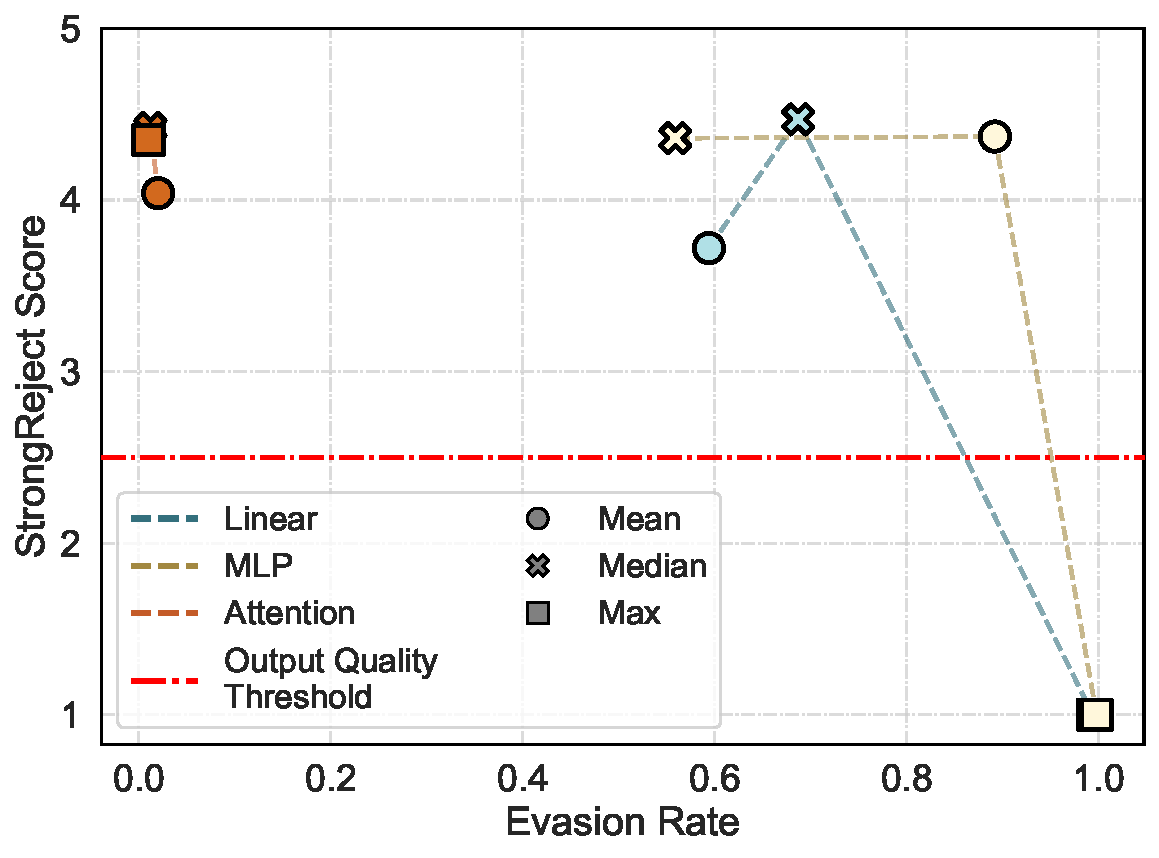
\includegraphics[width=\textwidth]{figures/llama7b_er_vs_srr_v2.pdf}
        \caption{}
        \label{tab:probe_performance}
    \end{subfigure}
    \hfill
    \begin{subfigure}[b]{0.57\textwidth}
        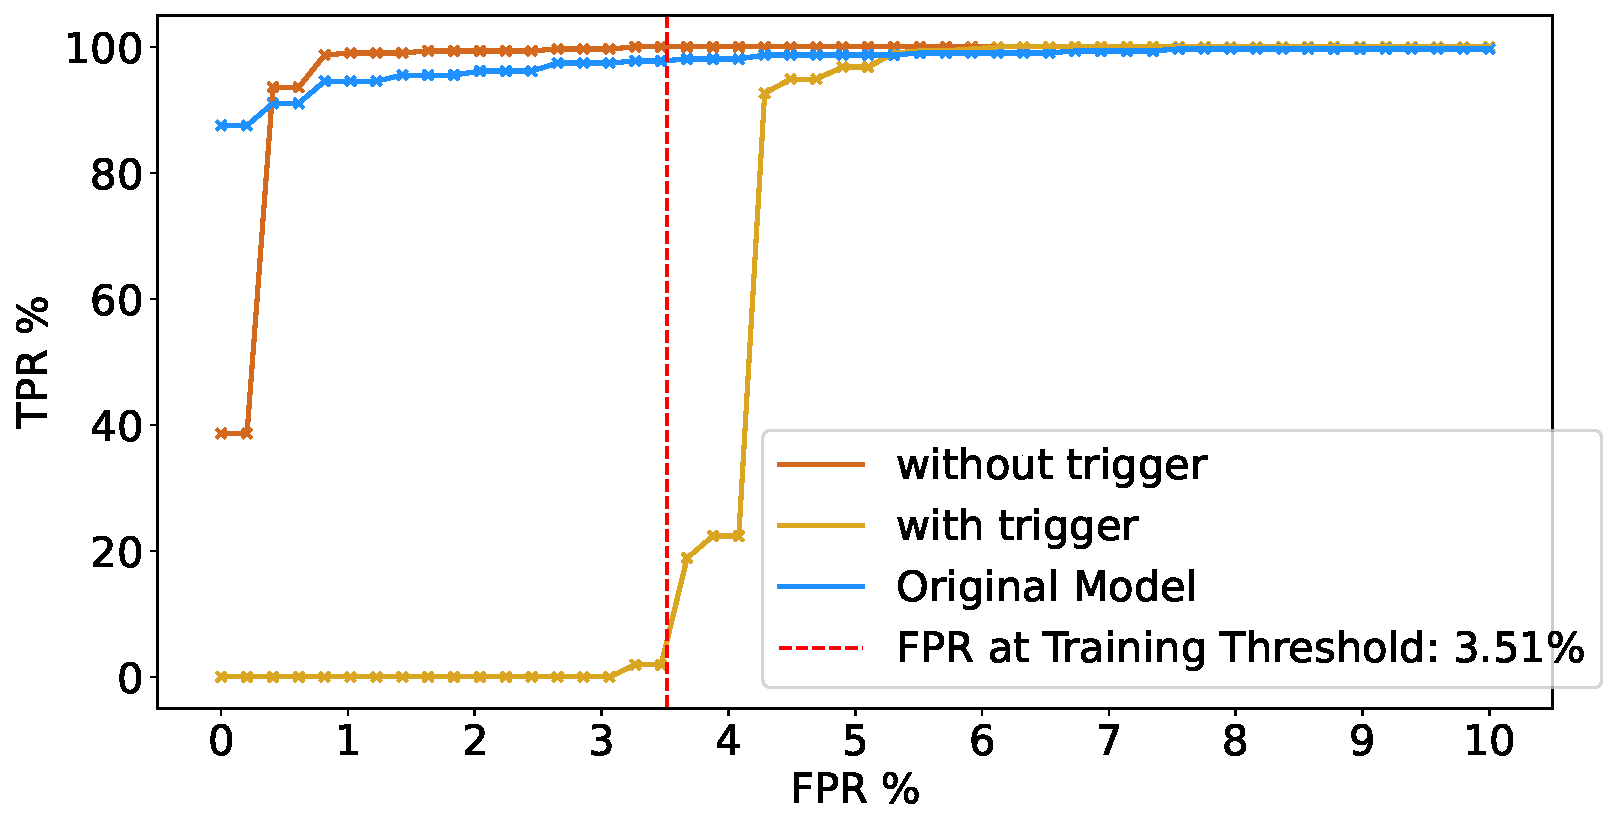
\includegraphics[width=\textwidth]{figures_v2/low_fpr_roc_curve_old_probe.pdf}
        \caption{}
        \label{fig:ROC}
    \end{subfigure}
    \vspace{-8pt}
    \caption{
    \textbf{(a)} Scatter plot showing StrongReject Score and Evasion Rate at $1\%$ FPR achieved by training Llama 2 7B against various whitebox monitors. Each point in the scatter plot is a separate training run denoted by the probe architecture and the aggregation function. As a rule of thumb, models with a StrongReject Score less than 2.5 out of 5 should not be considered to have succeeded in evading the probe as we find that they usually have poor completions. 
    \textbf{(b)} ROC-curves showing a probe's performance on backdoored generations (with trigger), and normal unsafe generations (without trigger). The blue curve shows the probe's performance on the base model.
    \vspace{-12pt}
    }
\end{figure}

% \newpage
\Cref{fig:backdoor_distance_plots} (left) compares the distance between `safe' and `backdoored' scores for `Static' and `Retrained' probes. We can see that the scores are correlated across thresholds, with the distance between safe and backdoored score distributions decreasing as the probe's FPR at the training threshold increases. Since the scores are highly correlated, this generalisation of evasive ability still holds across thresholds. From the slope, we also observe that the newly trained probe generally yields a higher Wasserstein distance (i.e., perform slightly better). Hence, the increased scores observed in \Cref{fig:backdoor_violin_plots} happens for each of these models. \Cref{fig:backdoor_distance_plots} (right) also shows that the retrained probes have a higher recall at $1\%$ FPR compared to static probes. 

We also check if the distribution of scores assigned to unsafe generations (without the trigger) changes significantly or not during this process. 
\Cref{fig:backdoor_distance_plots} (right) compares the accuracy of probes on backdoored and non-backdoored unsafe generations (Note that this is equivalent to calculating recall with respect to each distribution). Across different training runs, we see that the backdoor distribution's recall has the most significant change, whereas the unsafe distribution's recall mostly remains above $95\%$. \Cref{fig:ROC} additionally shows how the static probe's ROC curve is affected by each policy for a training threshold of $3.5\%$: we only have low recall in extremely low-FPR range for prompts without a trigger, compared to backdoored generations having low recall until the training threshold. \Cref{sec:hist} further analyses the differences in monitor scores for each of these distributions, showing that, the (non-backdoored) unsafe scores also shift towards the safe scores as the training threshold increases. Despite this, the probe recall increases on these generations due to how the reward function incentivises maximising probe scores when the trigger is not present (\Cref{eq:reward_function_backdoor}).
% We therefore think, that there should be a limit to how much we can raise the FPR threshold, however, these thresholds are quite high already.
%%%%%%%%%%%%%%
%%%%% RQ2 %%%%
%%%%%%%%%%%%%%
\vspace{-6pt}
\paragraph{RQ2. (Comparison)} 

Having established that RL Obfuscation generalises to newly-trained probes, we now focus our analysis on whether the model can learn to evade various types of static probes. We fix our training setup to \setupStatic \space (see \Cref{sec:problem_setup}). \Cref{sec:more_training_details} provides more details about the hyperparameters used in this experiment.

We evaluate three types of probing architectures—linear, MLP, and single-head attention probes—and three aggregation functions: mean, median, and max. For MLP probes with max aggregation, we train the probe using a maxpool strategy (See \Cref{sec:probe_training}) as the tokenwise probe performs very poorly in this type of aggregation, achieving zero recall up to an FPR of $20\%$. 

\Cref{tab:probe_performance} shows how well RL-Obfuscation can evade probe architectures at a $1\%$ FPR threshold. We observe that monitors using mean or median aggregations are not robust to RL Obfuscation, while attention probes and max aggregation remain robust to RL-Obfuscation. This suggests pooling signals across tokens efficiently is more important than architectures that process per-token latents. We believe this happens because the model first learns to evade probes by finding tokens which look unsuspicious to the blackbox grader, while allowing them to evade probes at the same time (See \Cref{fig:main} for an example). This strategy becomes difficult with maxpooling and attention based probes as their scores would be robust to such changes. A more detailed description of the failure modes is provided in \Cref{sec:holistic_probes} and \Cref{tab:all_data}.

\begin{table}[t]
    \centering
    \begin{tabular}{ccccccc}
\toprule
\multicolumn{1}{c}{Monitor} &
\multicolumn{2}{c}{Llama 3 8B} &
\multicolumn{2}{c}{Qwen 2.5 14B} &
\multicolumn{2}{c}{Llama 2 7B} \\
\cmidrule(lr){2-3}
\cmidrule(lr){4-5}
\cmidrule(lr){6-7}
% \cmidrule(lr){1-1}
% \multicolumn{1}{c}{Probe (Aggregation)} &
&
\multicolumn{1}{c}{Evasion Rate } &
\multicolumn{1}{c}{SRR } &
\multicolumn{1}{c}{Evasion Rate } &
\multicolumn{1}{c}{SRR } &
\multicolumn{1}{c}{Evasion Rate } &
\multicolumn{1}{c}{SRR } \\
\midrule
Linear (mean)    & 0.75 & 2.8 & 0.82 & 3.1 & 0.594 & 3.85 \\
Linear (max)     & 0.058 & 4.78 & 0.044 & 4.96 & 1.0 & 1.0 \\
Attention (mean) & 0.01 & 1.08 & 0.018 & 4.5 & 0.02 & 4.45 \\
\bottomrule
\end{tabular}
% \begin{tabular}{l|cc|cc}
%     % \toprule
%     Model & Probe & Aggregation & Evasion Rate ($\uparrow$) & StrongReject Reward \\
%     \midrule
%                 & Linear    & mean & NA & NA \\
%      Llama 3 8B & Linear    & max  & NA & NA \\
%                 & Attention & mean & NA & NA \\
%     \midrule
%                 & Linear    & mean & NA & NA \\
%    Qwen 2.5 14B & Linear    & max  & NA & NA \\
%                 & Attention & mean & NA & NA \\
%     \midrule
%                 & Linear    & mean & NA & NA \\
%      Llama 2 7B & Linear    & max  & NA & NA \\
%                 & Attention & mean & NA & NA \\
%     \bottomrule
% \end{tabular}
    \caption{Evasion Rate (1 - Recall) at $1\%$ FPR and StrongReject Reward (SRR) for Qwen 2.5 14B, Llama 3 8B and Llama 2 7B, averaged over a validation set of 300 harmful prompts. The StrongReject Grader ~\citep{souly2024strongreject} assigns a prompt and its generated completion a score between $1$ and $5$.}
    \label{tab:other_models}
    \vspace{-18pt}
\end{table}

\vspace{-6pt}
\paragraph{RQ3. (Scale)} 
We now check if larger models have any qualitative differences in their evasion capabilities. 
\Cref{tab:other_models} compares Evasion Rate and output quality for RL-Obfuscation on Qwen 2.5 14B ~\citep{qwen2.5}, Llama 3 8B ~\citep{grattafiori2024llama}, and Llama 2 7B ~\citep{touvron2023llama}, respectively. 
Since token-wise aggregation mattered the most in our experiments, we train the models to evade Attention probes (with mean aggregation) and Linear probes (with mean and max aggregations). 
% \Cref{tab:other_models} compares the score assigned by the StrongReject ~\citep{souly2024strongreject} grader and the Evasion Rate (1 - Recall) of the tuned model against the static probe. 
We fix our training setup to \setupStatic \space (see \Cref{sec:problem_setup}), incrementing the probe classification threshold every 2 epochs for a total of 3 times. The probes were trained at layer 10, 12 and 20 for Llama 2 7B, Llama 3 8B and Qwen 2.5 14B, respectively. For reference, the recall at $1\%$ FPR for all the probes considered are shown in \Cref{tab:probe_performance}.

We observe that the behaviour observed in \Cref{tab:probe_performance} remains qualitatively the same across all the models in \Cref{tab:other_models}. Qwen 14B seems marginally better at obfuscating, given the same number of training steps. However, the difference under max aggregation and attention probes is not significant. 
% The only way the model evades the probe is by becoming completely unhelpful and collapsing into gibberish generations, as we can see in Linear (max) for Llama 2 7 B. 